\section{Exercise 11}
notes
a = learningrate
e = exploration/mutation rate
y = discount rate

newQ = (1 - a)oldQ + (a)sample
sample = reward + y(futureQs)
if random < e: random step
else best step
\subsection{}
Testing method(also for 11.b):
I let the the crawler walk until he disappears from the screen at the end.
That is one run. I measure the run time in ticks. I take 8 runs.
The runs are consecutive.

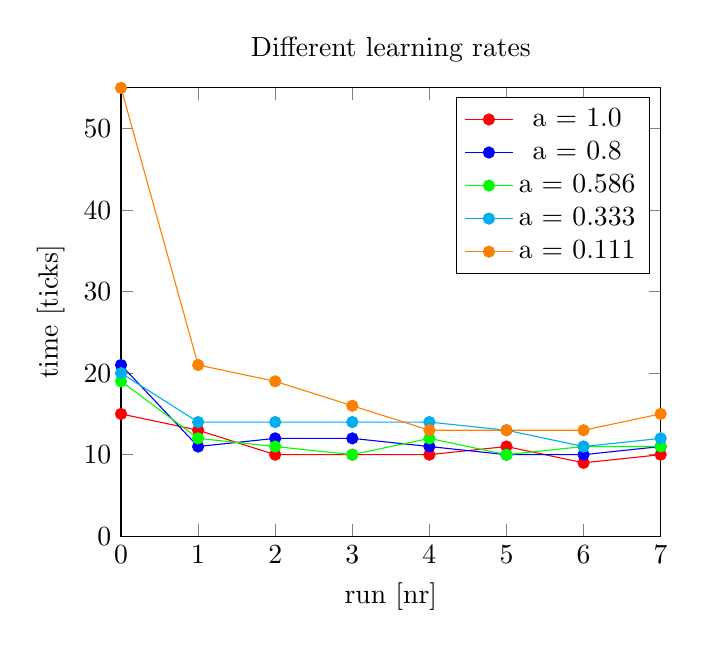
\begin{tikzpicture}
\begin{axis}[
    title={Different learning rates},
    xlabel={run [nr]},
    ylabel={time [ticks]},
    xmin = 0, xmax = 7,
    ymin = 0, ymax = 55
]
\addplot[
    color=red,
    mark=*
]
coordinates{(0,15)(1,13)(2,10)(3,10)(4,10)(5,11)(6,9)(7,10)};
\addplot[
    color=blue,
    mark=*
]
coordinates{(0,21)(1,11)(2,12)(3,12)(4,11)(5,10)(6,10)(7,11)};
\addplot[
    color=green,
    mark=*
]
coordinates{(0,19)(1,12)(2,11)(3,10)(4,12)(5,10)(6,11)(7,11)};
\addplot[
    color=cyan,
    mark=*
]
coordinates{(0,20)(1,14)(2,14)(3,14)(4,14)(5,13)(6,11)(7,12)};
\addplot[
    color=orange,
    mark=*
]
coordinates{(0,55)(1,21)(2,19)(3,16)(4,13)(5,13)(6,13)(7,15)};
\legend{a = 1.0, a = 0.8, a = 0.586, a = 0.333, a = 0.111}
\end{axis}
\end{tikzpicture}

The higher the learningrate, the faster the crawler's policy 
converges. But, lower learningrate's do not slow the process of 
learning down much, till a certain point. After that the learning 
speed is affected significantly, as you can see with the orange line 
in the graph. Eventually they will converge, sooner or later. 

\subsection{}

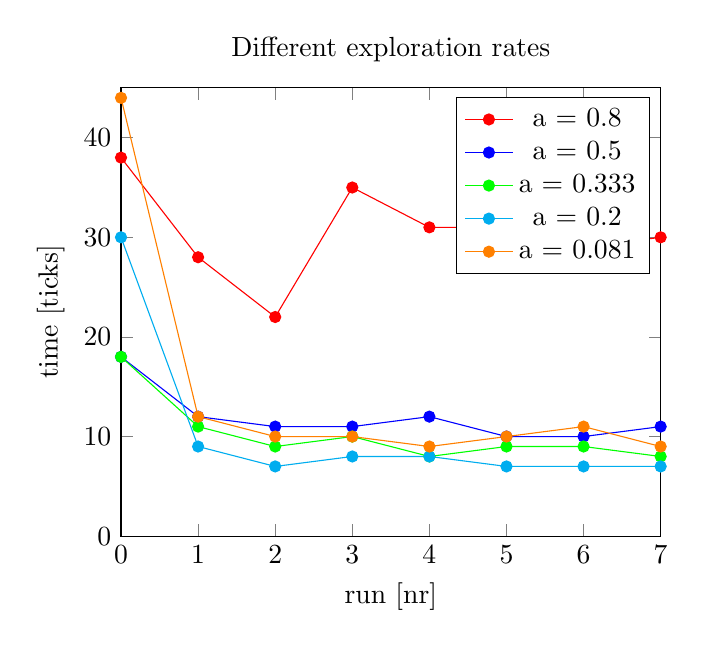
\begin{tikzpicture}
\begin{axis}[
    title={Different exploration rates},
    xlabel={run [nr]},
    ylabel={time [ticks]},
    xmin = 0, xmax = 7,
    ymin = 0, ymax = 45
]
\addplot[
    color=red,
    mark=*
]
coordinates{(0,38)(1,28)(2,22)(3,35)(4,31)(5,31)(6,29)(7,30)};
\addplot[
    color=blue,
    mark=*
]
coordinates{(0,18)(1,12)(2,11)(3,11)(4,12)(5,10)(6,10)(7,11)};
\addplot[
    color=green,
    mark=*
]
coordinates{(0,18)(1,11)(2,9)(3,10)(4,8)(5,9)(6,9)(7,8)};
\addplot[
    color=cyan,
    mark=*
]
coordinates{(0,30)(1,9)(2,7)(3,8)(4,8)(5,7)(6,7)(7,7)};
\addplot[
    color=orange,
    mark=*
]
coordinates{(0,44)(1,12)(2,10)(3,10)(4,9)(5,10)(6,11)(7,9)};
\legend{a = 0.8, a = 0.5, a = 0.333, a = 0.2, a = 0.081}
\end{axis}
\end{tikzpicture}

The exploration rate let the crawler take random actions to discover 
new things. A high exploration rate will never be fast. Even if the 
agent has tried many things and learned the optimal policy from it, 
it will still perform random actions instead of the learned ones. 
As you can see with the red line, the time of completion stays high. 
Lowering the exploration rate let the crawler move faster due to less 
random moves, but if we drop it to low it will learn less fast. We 
can see that lower rates do better, for all except the lowest value here.
We can see that the orange line is consistently above the cyan line, 
breaking the trend. Many more tests may reveal a optimal learning rate 
somewhere between cyan and orange.

\subsection{}

high a(learningrate), low e(explorationrate) = learns fast from actions performered, but tries little new things.
Since he does not know anything to start with, he needs to randomly come across a good action at the right time.
The low e value holds the crawler back from learning as fast as he could.

high a, high e = learns fast from actions performered, and also tries many things(random) out.
This combination lets the crawler learn rapidly at the beginning. However, when he has learned to walk, the high e
holds him back from performing at his best. Because a high e brings a high probability for a random action, his
behaviour is quite random. Now he knows the right actions, this is not needed anymore. Many steps are now wasted, the random
actions do not contribute walking faster and could even push him back at bit.

low a, low e = This is a very slow learning combination. There is a low chance that he will randomly do something.
And if he randomly does something right, it picks it up slow because of the low a. But when it, eventually, learned how to walk
he performs great. He will not disrupt his walk with randomness, and random bad actions do not influence him because of
the low a.

low a, high e = This one is weird. He tries many things, but learns from them slowly. When he learned to crawl, randomness
still disrupts his speed. But this time it will not affect the learned policy so much.

The best thing is to have a high e and a high a, so he learns fast. He will start walking in no time. Then you can decrease
the e and a slowly as he gets better. At the end set them to zero as the learning has finalised. Then there will be no
randomness to disrupt the crawl, and the crawler will be at his fastest.

\subsection{}

\subsection{}